\contribution{Central Processing Unit}
\shortcontributor{CS6230 : CAD for VLSI Project Report}
\shortcontribution{Overview}
\headnum{2}
\begin{paper}
\renewcommand*{\pagemark}{}

\section*{}


\begin{figure}[H]
\centering
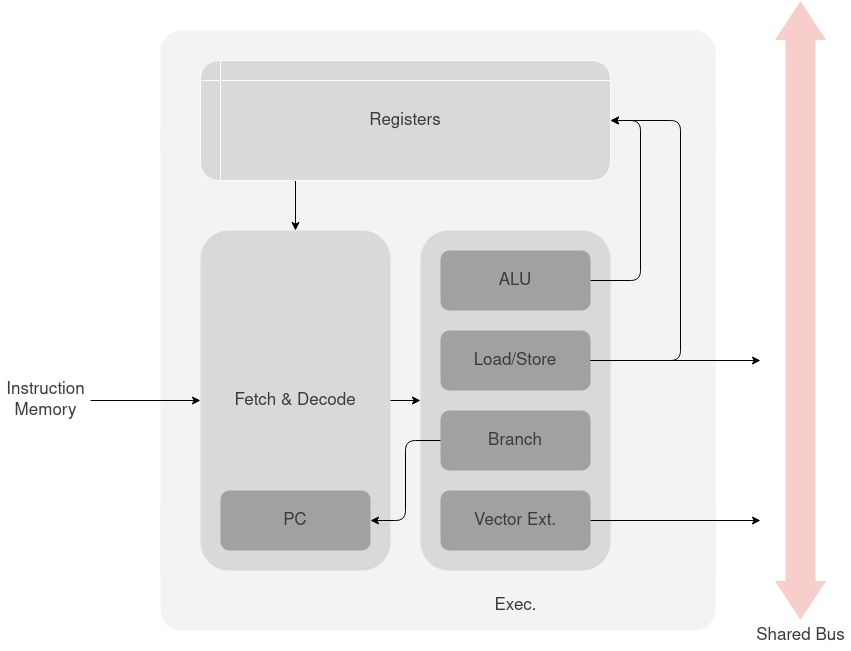
\includegraphics[width=10cm]{Images/Overview-CPU(1).png}
\caption{\content Architecture of the CPU.}
\end{figure}

\nointend We designed a minimal 2 stage pipelined CPU capable of doing basic arithmetic, logic, memory load/store, and custom vector operations. The instruction memory is separated from the data memory. Instructions will be issued in order. For branches, the fetch stage will be flushed, and the program counter will be updated. In the case of vector instructions, the appropriate CSRs of the corresponding accelerators will be updated accordingly. The general architecture of the CPU is as given in the figure.
\section*{The Registers\sdot}
Our CPU consists of 8 general-purpose registers R0, R1, R2, ... R7. The capacity of the registers is parameterized. However, our current instruction set supports only 8, 16, and 32-bit values and operations on them. According to the instruction, an individual physical register can be perceived as an 8-bit, a 16-bit, or a 32-bit register. For instance, \texttt{ASG\_8 R1 4} will consider only the lower 8 bits of R1, whereas \texttt{ASG\_15 R1 4} will consider the lower 16 bits.
\begin{figure}[H]
\centering
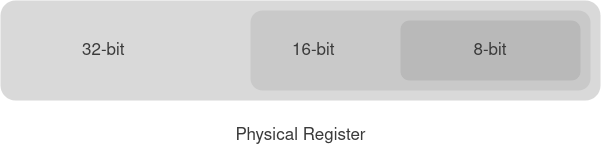
\includegraphics[width=8cm]{Images/Overview-Registers.png}
\caption{\content The same register RX can be perceived as 8, 16 or 32-bit register.}
\end{figure}

\section*{The Instruction Set\sdot}
\begin{figure}[H]
\centering
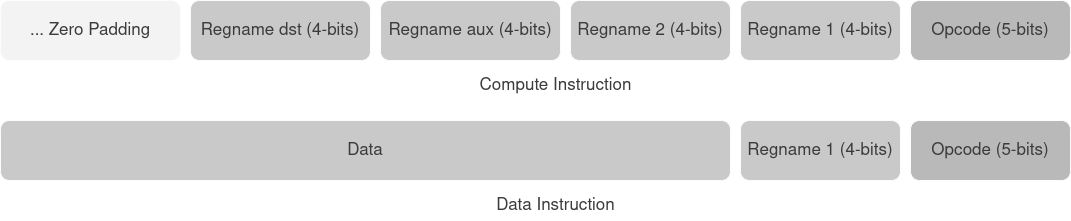
\includegraphics[width=11cm]{Images/Overview-InstructionSet.png}
\caption{\content Structure of the instructions.}
\end{figure}
We devised a minimal custom ISA capable of basic arithmetic, logic, branch, load/store, and custom vector operations. The CPU's must have a minimum word length of 32 bits. The same instructions, padded with zeros, are used for CPUs of higher word lengths. All instructions except the 32-bit Assign instruction in 32-bit CPUs are of the same length equal to the word length. In this case, the instruction (\texttt{ASG\_32} in 32-bit CPU) is 64-bits long to accommodate the 32-bit value for Assign operation. Our custom ISA is as given below. A small assembler was written in Python to generate machine code in a format supported by Bluespec testbench.\\\\
\nointend To run the assembler,
\begin{minted}[
bgcolor=Gray !20
]{bash}
cd src/asm/
./asm input_file.asm -o output -w 64
\end{minted}
\nointend Where the \texttt{-w} argument is the wordlength of the CPU. The argument is optional and the default is as for a 32-bit CPU.


\begin{center}
\begin{longtable}{l l l l}
 \heavy Instruction & \heavy Opcode& \heavy Example & \heavy Description\\ 
NOP & 0x00 & NOP & No op \\  
ASG\_8 & 0x01 & AGS\_8 R1 11 & Assigns int8 11 to Register R1 \\
ASG\_16 & 0x02 & ASG\_16 R1 11 & Assigns int16 int 11 to Register R1 \\
ASG\_32 & 0x03 & ASG\_32 R1 11 & Assigns int32 int 11 to Register R1 \\
&&ASG\_32 R1 11.0 & Assigns float32 11.0 to Register R1 \\
MOV & 0x04 & MOV R1 R2 & Moves content of R1 to R2\\
ADD\_I8 & 0x05 & ADD\_I8  R1 R2 R3 & int8 addition R3 <- R1 + R2\\
ADD\_I16 & 0x06 & ADD\_I16  R1 R2 R3 & int16 addition R3 <- R1 + R2\\
ADD\_I32 & 0x07 & ADD\_I32  R1 R2 R3 & int32 addition R3 <- R1 + R2\\
ADD\_F32 & 0x08 & ADD\_F32  R1 R2 R3 & float32 addition R3 <- R1 + R2\\
SUB\_I8 & 0x09 & SUB\_I8  R1 R2 R3 & int8 addition R3 <- R1 + R2\\
SUB\_I16 & 0x0a & SUB\_I16  R1 R2 R3 & int16 addition R3 <- R1 - R2\\
SUB\_I32 & 0x0b & SUB\_I32  R1 R2 R3 & int32 addition R3 <- R1 - R2\\
SUB\_F32 & 0x0c & SUB\_F32  R1 R2 R3 & float32 addition R3 <- R1 - R2\\
IS\_EQ & 0x0d & IS\_EQ  R1 R2 R3 & R3 <- (R1 == R2)\\
JMP & 0x0e & JMP R1 & Jump PC to address pointed by R1\\
JMPIF & 0x0f & JMPIF R1 R2 & Jump to address R1 if R2 is true\\
LOAD\_8 & 0x10 & LOAD\_8 R1 R2 & Load 8-bits from address pointed\\
&&& by R1 to R2\\
LOAD\_16 & 0x11 & LOAD\_16 R1 R2 & Load 16-bits from address pointed\\
&&& by R1 to R2\\
LOAD\_32 & 0x12 & LOAD\_32 R1 R2 & Load 32-bits from address pointed\\
&&& by R1 to R2\\
STORE\_8 & 0x13 & STORE\_8 R1 R2 & Store 8-bits R1 to address pointed\\
&&& by R2\\
STORE\_16 & 0x14 & STORE\_16 R1 R2 & Store 16-bits R1 to address pointed\\
&&& by R2\\
STORE\_32 & 0x15 & STORE\_32 R1 R2 & Store 32-bits R1 to address pointed\\
&&& by R2\\
VEC\_NEG\_I8 & 0x16 & VEC\_NEG\_I8 R1 R2 R3 & Bit wise negation of int8 vector\\
&&& starting pointed by R1, length R2,\\
&&& and store back to address in R3\\
VEC\_NEG\_I16 & 0x17 & VEC\_NEG\_I16 R1 R2 R3 & Bit wise negation of int16 vector\\
&&& starting pointed by R1, length R2,\\
&&& and store back to address in R3\\
VEC\_NEG\_I32 & 0x18 & VEC\_NEG\_I31 R1 R2 R3 & Bit wise negation of int32 vector\\
&&& starting pointed by R1, length R2,\\
&&& and store back to address in R3\\
VEC\_NEG\_F32 & 0x19 & VEC\_NEG\_F32 R1 R2 R3 & Bit wise negation of float32 vector\\
&&& starting pointed by R1, length R2,\\
&&& and store back to address in R3\\
VEC\_MIN\_I8 & 0x1a & VEC\_MIN\_I8 R1 R2 R3 & Statistics minimum of int8 vector\\
&&& starting pointed by R1, length R2,\\
&&& and store back to address in R3\\
VEC\_MIN\_I16 & 0x1b & VEC\_MIN\_I16 R1 R2 R3 & Statistics minimum of int16 vector\\
&&& starting pointed by R1, length R2,\\
&&& and store back to address in R3\\
VEC\_MIN\_I32 & 0x1c & VEC\_MIN\_I31 R1 R2 R3 & Statistics minimum of int32 vector\\
&&& starting pointed by R1, length R2,\\
&&& and store back to address in R3\\
VEC\_MIN\_F32 & 0x1d & VEC\_MIN\_F32 R1 R2 R3 & Statistics minimum of float32 vector\\
&&& starting pointed by R1, length R2,\\
&&& and store back to address in R3\\
\end{longtable}
\end{center}


\section*{The Fetch and Decode Stage\sdot}
The fetch stage fetches the instructions from the instruction memory, checks for any data dependencies, and looks up the data required for computation from the registers, and enqueues to decoded instruction to the execute stage. In the case of any data dependencies, a \texttt{NOP} is sent into the execute stage. \\\\
\nointend All the data instructions (the assignment instructions) are processed in the fetch stage. This architecture creates a conflict if the execute stage tries to store a value to the same register. The data instruction from the fetch stage is given priority for resolving the conflict. In other words, during a consecutive write after write (WAW) dependency, the first write is disregarded.\\\\
\nointend The fetch stage is also responsible for decomposing complex vector instructions to a sequence of load/store instructions. For example, the \texttt{VEC\_NEG\_I8} instruction is broken down into a stream of store instructions that stores the pointers to the data to the memory-mapped accelerator and triggers the accelerator. This process creates overhead on the CPU. A potential alternative is for the compiler to decompose the vector functions and keep the individual instructions short. However, this method results in more large programs. 

\section*{The Execute Stage\sdot}
Since being an inorder processor, the execute stage is relatively straight forward. The opcode is used to send the instructions to the right unit. In the case of a branch, the pipeline is flushed. There is no value forwarding to the fetch stage, and the instructions with data dependencies are kept awaiting. There is also no value forwarding between store and load operations. \\\\
\nointend For vector instructions, the fetch stage already decomposes the instructions into the corresponding load/store transactions. Therefore the execute stage executes these instructions, idles and pings the accelerator to check for the completion of the instruction. The length of the vector determines the frequency of pings. The pings must not be excessively frequent as it consumes the expensive bus ownership time that the accelerators require, and the pings must not be over sparse as this results in the CPU holding idle for long.
\end{paper}